\chapter{User Flows}
\label{ch:user-flows}

\section{CLI journey}

\begin{figure}[H]
\centering
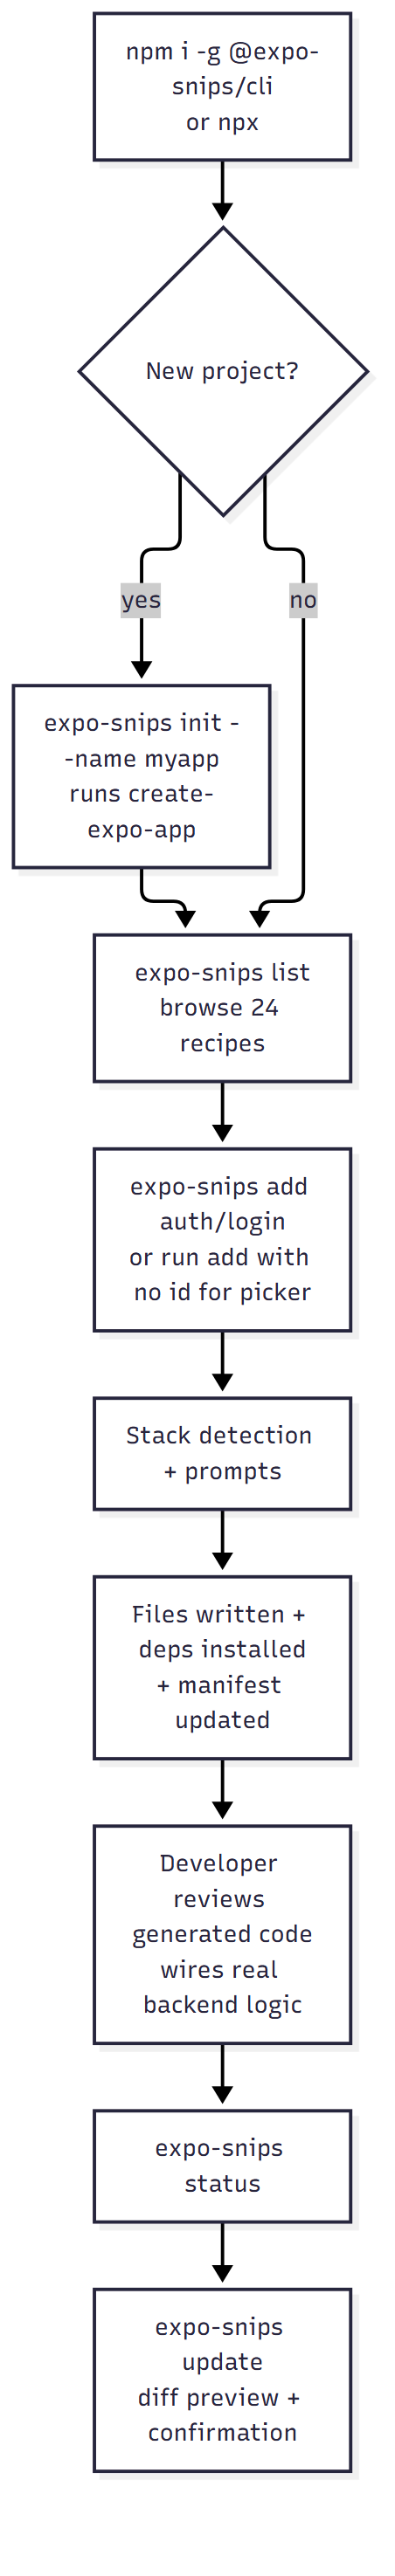
\includegraphics[width=0.92\textwidth]{diagrams/user-flow-cli.png}
\caption{CLI journey from installation to keeping screens up to date}
\label{fig:user-flow-cli}
\end{figure}

\begin{longtable}{p{1cm}p{4.2cm}p{9.2cm}}
\caption{CLI journey steps}\\
\toprule
\textbf{\#} & \textbf{Step} & \textbf{Detail} \\
\midrule

1 & Install & \texttt{npm i -g @expo-snips/cli}, or invoke through \texttt{npx}. \\
2 & (Optional) bootstrap & \texttt{expo-snips init --name myapp} runs
\texttt{create-expo-app}. \\
3 & Browse & \texttt{expo-snips list} prints 24 recipes with tags. \\
4 & Generate & \texttt{expo-snips add auth/login} (or bare \texttt{add} for a picker). \\
5 & Detect and prompt & The CLI reports detected values and prompts only for
unresolved options. \\
6 & Write and install & Files are created; recipe dependencies are installed. \\
7 & Record & \texttt{.expo-snips.json} is updated. \\
8 & Review & The developer edits the generated code and wires real logic. \\
9 & Maintain & \texttt{status} to inspect, \texttt{update} to pull catalog
improvements with a diff preview. \\
\bottomrule
\end{longtable}

\section{VS Code journey}

\begin{figure}[H]
\centering
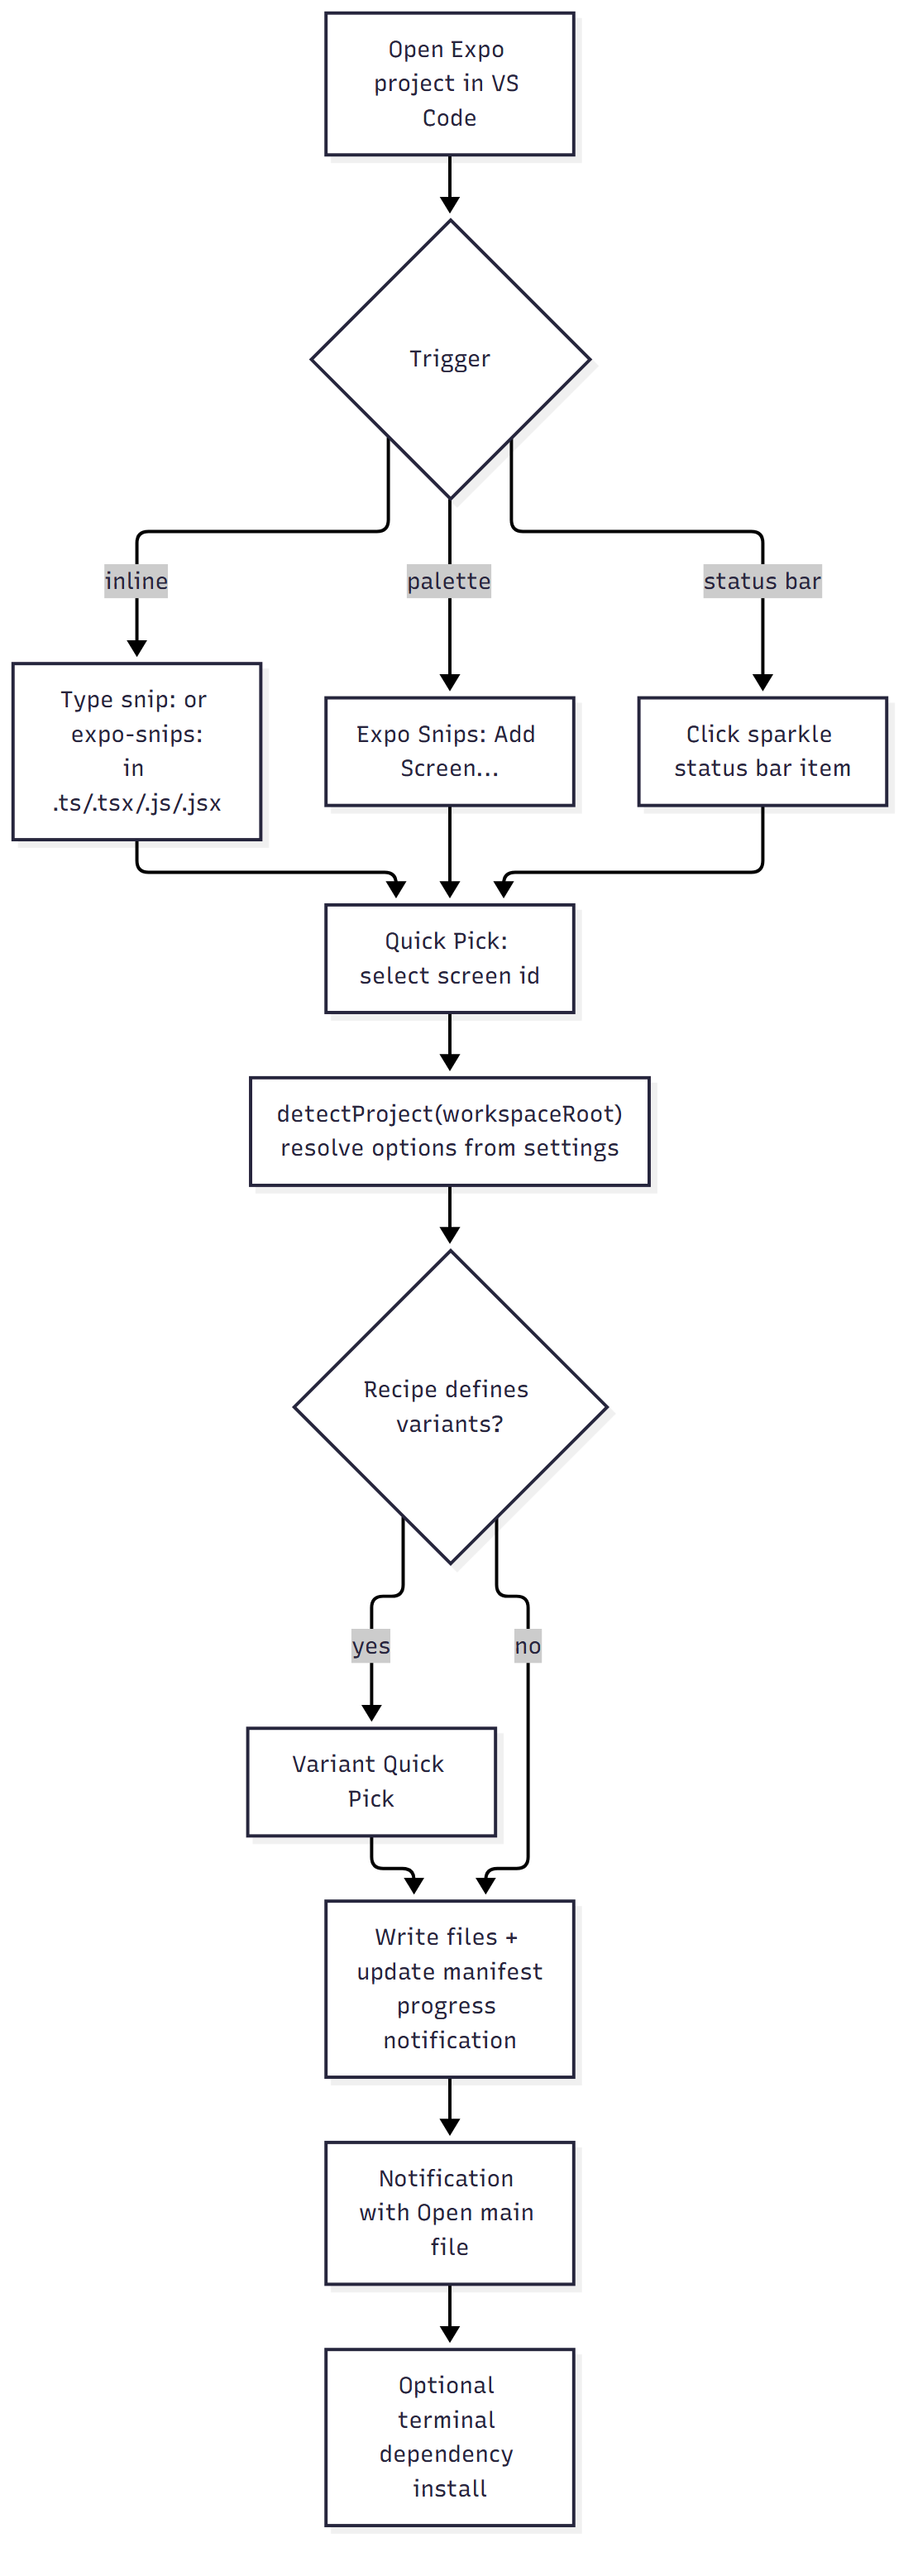
\includegraphics[width=0.9\textwidth]{diagrams/user-flow-vscode.png}
\caption{VS Code journey using the inline completion trigger}
\label{fig:user-flow-vscode-ux}
\end{figure}

\begin{longtable}{p{1cm}p{4.2cm}p{9.2cm}}
\caption{VS Code journey steps}\\
\toprule
\textbf{\#} & \textbf{Step} & \textbf{Detail} \\
\midrule

1 & Open a project & The extension activates on a TS/JS language or the command. \\
2 & Trigger & Type \texttt{snip:} or \texttt{expo-snips:}; or run ``Expo Snips: Add
Screen...''; or click the status bar item. \\
3 & Select & A Quick Pick lists recipe names with ids and descriptions. \\
4 & Resolve & Options are computed silently from detection and settings; a variant
Quick Pick appears only when the recipe declares variants. \\
5 & Generate & Files are written under a progress notification. \\
6 & Complete & An information message reports the file count and offers ``Open main
file''. \\
7 & Install & Dependencies are installed in an ``Expo Snips'' terminal when the
setting is enabled. \\
\bottomrule
\end{longtable}

\section{Variant selection flow}

\begin{enumerate}
  \item The CLI accepts \texttt{--variant glass}. For a recipe without a glass
        variant, the flag is accepted and the default template is used.
  \item In VS Code, \texttt{pickVariant} returns undefined when
        \texttt{recipe.variants} is empty; otherwise it shows a Quick Pick of
        variant labels and returns the selected id.
  \item During rendering, \texttt{resolveTemplateString} prefers the variant
        template over the default for that file entry.
\end{enumerate}

Only \texttt{app/home}, \texttt{auth/login} and \texttt{onboarding/welcome} define
variants, so the variant Quick Pick appears only for those three recipes.

\section{Update flow}

The update flow is documented as a state machine in Chapter~\ref{ch:data-flows}
(Figure~\ref{fig:update-flow}).

\section{Error and recovery flows}

\begin{longtable}{p{4.2cm}p{5cm}p{5.2cm}}
\caption{Recovery flows}\\
\toprule
\textbf{Situation} & \textbf{What the user sees} & \textbf{Recovery} \\
\midrule

Typo in screen id & ``Screen not found: <id>'' and a pointer to \texttt{list}. & Run
\texttt{list} and retry. \\
Unsupported option & ``Recipe "..." does not support <option> "...".'' & Omit the
flag; the tool will detect or prompt. \\
No files matched & ``No files matched the selected options. Nothing generated.'' &
Choose an option combination the recipe supports (check \texttt{list} output or
the recipe document). \\
Registry unreachable & CLI warning: ``Could not reach registry at <base>. Using N
built-in screens.'' & Remove or correct the registry base; generation continues
from the embedded catalog. \\
Option cancelled mid-prompt & Silent exit with code 1. & Re-run and complete the
prompts. \\
Update declined & ``Update cancelled.'' & Re-run when ready; nothing was written. \\
No manifest & ``No screens tracked in this project yet.'' & Run \texttt{add} first. \\
\bottomrule
\end{longtable}
